%%% Local Variables:
%%% mode: Xelatex
%%% TeX-master: t
%%% End:

\documentclass[draftformat,mathtimes]{HUSTthesis}%草稿用这个
%\documentclass[finalformat,mathCMR]{HUSTthesis}%盲审用这个
\raggedbottom %顶端对齐,避免LaTeX在特定情况下自动增大段间距

\usepackage{HUSTtils}% 所有其它可能用到的包都统一放到这里了,可以根据自己的实际添加或者删除。这样做主要是为了避免class文件过于臃肿。
% \setmainfont{Times New Roman}[Scale=.9]
\setmainfont{Times New Roman}
%\includeonly{body/chap02}
\begin{document}

%定义所有的eps文件在 figures 子目录下
\graphicspath{{figures/}}

% 生成封面,版权页,摘要

\frontmatter

%%% Local Variables:
%%% mode: Xelatex
%%% TeX-master: t
%%% End:

\ctitle{标题:宋体,英文 Times New Roman,一号,加粗,不超 30 字\\
\textcolor{red}{中英文标题、学科专业、导师姓名正确、一致}}

\xuehao{D2019xxxxx} \schoolcode{10487}
\csubjectname{XXXXX} \cauthorname{XXX}
\csupervisorname{XXX} \csupervisortitle{教授}
\defencedate{202X~年~X~月~X~日} \grantdate{}
\chair{}%
\firstreviewer{} \secondreviewer{} \thirdreviewer{}

\etitle{English Title,Times New Roman,小二号,实词的首字母大写\\
\textcolor{red}{中英文标题、学科专业、导师姓名正确、一致}}
\edegree{Doctor of Engineering}
\esubject{Control Science and Engineering}
\eauthor{(中文习惯,姓在前且姓全部大写)}
\esupervisor{Prof. xxx}
\edate{May, 2022}

%定义中英文摘要和关键字
\cabstract{

摘要是学位论文极为重要、不可缺少的组成部分,它是论文的窗口,并频繁用于国内外资料交流、情报检索、二次文献编辑等。其性质和要求如下:\par
    [1] 摘要即摘录论文要点,是论文要点不加注释和评论的一篇完整的陈述性短文,具有很强的自含性和独立性,能独立使用和被引用。\par
    [2] 博士学位论文的摘要应包含全文的主要信息,并突出创造性成果。\par
    [3] 内容范围应包含以下基本要素:\par
    \hspace{1em}(1) 目的:研究、研制、调查等的前提、目的和任务以及所涉及的主题范围。\par
    \hspace{1em}(2) 方法:所用原理、理论、条件、对象、材料、工艺、手段、装备、程序等。\par
    \hspace{1em}(3) 结果:实验的、研究的、调查的、观察的结果、数据,被确定的关系,得到的效果、性能等。\par
    \hspace{1em}(4) 结论:结果的分析、研究、比较、评价、应用;提出的问题,今后的课题,建议,预测等。\par
    \hspace{1em}(5) 其他:不属于研究、研制、调查的主要目的,但就其见识和情报价值而言也是重要的信息。\par
    [4] 摘要的详简度视论文的内容、性质而定,\textcolor{red}{博士学位论文摘要一般为800-1000汉字。}\par
    [5] 摘要及全文中均不得出现“我们”等字样。一般不用图、表、化学结构式、计算机程序,不用非公知公用的符号、术语和非法定的计量单位。\par
    [6] 摘要中一般不使用缩写词,若实在需要,在第一次使用前,需给出中文全称(缩写词);在使用英文缩写词之前,需给出中文全称(英文全称,缩写词),再次出现时可以采用中文或英文缩写词。\par
    [7] \textcolor{red}{关键词应有3至8个,另起一行置于摘要下方,领域从大到小排列。关键词之间用分号隔开,最后一个关键词后面无标点。}\par
    [8] 摘要、关键词采用中文宋体;英文Times New Room;小四号;}


\ckeywords{关键词1;关键词2;关键词3}

\eabstract{This is abstract. 

英文摘要字体为Times New Roman,小四,1.5倍行距。

\textcolor{red}{英文摘要和关键词应与中文相对应。}英语摘要用词应准确,使用本学科通用的词汇;摘要中主语(作用)常常省略,因而一般使用被动语态;应使用正确的时态,并要注意主、谓语的一致,必要的冠词不能省略。}

\ekeywords{Keyword1, Keyword2, Keyword3}

\makecover

%目录
\tableofcontents

% 对照表
\begin{denotation}
\item[xue] 我的姓
\item[ruini] 我的名
\item[W.M. Zheng]  我的老师
\item[Tsinghua] 学校名
\item[Long] 来个比较长的,看看会出现什么情况。
\item[劝  学] 君子曰:学不可以已。青,取之于蓝,而青于蓝;冰,水为之,而寒于水。
  木直中绳。(车柔)以为轮,其曲中规。虽有槁暴,不复挺者,(车柔)使之然也。故木
  受绳则直, 金就砺则利,君子博学而日参省乎己,则知明而行无过矣。吾尝终日而思
  矣,  不如须臾之所学也;吾尝(足齐)而望矣,不如登高之博见也。登高而招,臂非加
  长也,  而见者远;  顺风而呼,  声非加疾也,而闻者彰。假舆马者,非利足也,而致
  千里;假舟楫者,非能水也,而绝江河,  君子生非异也,善假于物也。积土成山,风雨
  兴焉;积水成渊,蛟龙生焉;积善成德,而神明自得,圣心备焉。故不积跬步,无以至千
  里;不积小流,无以成江海。骐骥一跃,不能十步;驽马十驾,功在不舍。锲而舍之,朽
  木不折;  锲而不舍,金石可镂。蚓无爪牙之利,筋骨之强,上食埃土,下饮黄泉,用心
  一也。蟹六跪而二螯,非蛇鳝之穴无可寄托者,用心躁也。\pozhehao{} 荀况
\end{denotation}
  

\mainmatter
%%% mode: latex
%%% TeX-master: t
%%% End:

\chapter{绪论}
\label{cha:intro}

博士学位论文应能表明作者确已在本门学科上掌握了坚实宽广的基础理论和系统深入的专门知识,并具有独立从事科学研究工作的能力,在科学或专门技术上做出了创造性的成果。博士学位论文的字数一般不少于5万字,加上各类图表,从绪论到总结与展望的总页数一般不少于90页。否则,可能显得工作量不够饱满。

学位论文题名是以最恰当、最简明的词语反映论文中最重要的特定内容的逻辑组合。题名既要准确地描述内容,又要尽可能地精练,一般不宜超过30个字。题名一般避免使用不常见的缩略词、字符、代号和公式等。若实属必要,需要摘要中给出中英文全称与缩写。学位论文内容应结构合理、立论正确、推理严谨、文字简练、层次分明、逻辑严密、数据真实可靠。

学位论文文字排版的字号、行距、字距的大小,以版面清晰、容易辨识和阅读为原则。为统一起见,具体要求如下:
\begin{enumerate}
    \item 论文页眉,楷体,小二;
    \item 章和节的题名用黑体,字号分别用三号和四号;
    \item 正文内容用宋体,英文用Times New Roman,小四号;行间距1.5倍;正文注意两侧对齐。
\end{enumerate}

绪论部分是整篇论文的导引,应包括选题背景、意义;国内外研究概况;前人研究中存在的问题或知识空白;进而引出本文的研究设想,简要给出全文各章节的主要内容、以及章节之间相互联系。

在写作中无论是研究背景及意义,还是国内外研究现状,要做到有依据都必须引用参考文献。通常情况下,绪论部分的参考文献应占全文参考文献的百分之80以上。参考文献的顺序必须是按照在文章中出现的先后顺序进行排列。

以下简要说明一下绪论部分的内容及各级标题格式等。


\section{***的研究背景与意义}
\label{sec:general intro}
主要介绍与本文相关的基础知识,包括基本概念、理论、原理、方法与技术等,指出相关领域研究工作的意义。

在写作上要深入浅出,图文并茂,以便大同行也能读懂。


\subsection{**概念}



\subsection{**技术}



\section{XXX国内外研究现状}
\label{sec:requirement}

此处应就与本文相关的国内外研究概况进行全面综述,这样相关内容在后面章节中就可以点到为止,无需再大段大段地分别介绍了。

\section{存在的问题}
\label{sec:compile}

\section{研究内容}
\label{sec:xelatex}
不同学科、不同专业、不同学生学位论文的类别各异,大致可分为实验研究类、理论/算法研究类、仪器/工艺设计与研发类、综合类等。不同论文的章节结构各异,但每种类型的论文还是有其特定的格式。原则上,博士论文的主体研究内容不得少于3章,加上绪论、总结与展望,累计不得少于5章。

作为华中科技大学博士学位论文模板,本文首先给出了不同类型的研究论文典型结构供大家参考,再根据学术出版的规范化要求,说明论文写作中的细则。全文共分为5章。主要内容如下:

第1章 绪论:简要介绍论文的研究背景、国内外研究现状、存在的问题,给出全文的主要研究内容。为了让读者更容易理解全文,建议用一个文档结构图给出各章节逻辑关系。

第2章 样式使用说明:一般应介绍该章的主要内容,说明这一章做什么。

第3章 实验研究类论文:……

第4章 理论或算法类论文的结构:……

第5章 总结与展望:给出全文的主要内容及结论,总结本文的创新点,并对未来的工作进行展望。


%%% Local Variables:
%%% mode: latex
%%% TeX-master: t
%%% End:

\chapter{样式使用说明}
\label{cha:command}


\section{引言(引言标题可选)}
\label{sec:cover}
华中科技大学学位论文格式要求。

\section{导入自定义功能区}
为了方便使用,\textbf{添加“插入题注”和“插入交叉引用”等常用功能到word快速访问工具栏。}

(1)下载文件“Word 自定义.exportedUI”

(2)点击“WORD-文件-选项-自定义功能区-导入导出”,将文件“Word 自定义.exportedUI”导入。


\section{奇数页放置}
不要随意删除分节符、分页符。

(1)摘要、目录奇数页放置

(2)各章首页可以连续放置,需要加入分节符(下一页)

\section{各级标题}
输入文本内容,直接选择样式中对应的标题样式即可。

正文需要自定义手动添加二个字符缩进。


\section{图片表格自动编号与引用}
(1)制作图片或表格。

(2)点击图片或表格,选择样式“图标题”

(3)插入题注自动编号。题目推荐使用二个空格,不建议使用TAB空格(图目录不方便调节缩进)。

(4)交叉引用。在需要引用公式的地方用“插入”->“交叉引用”,选择引用类型和引用内容“只有标签和编号”交叉引用公式编号。如图\ref{Fig2-1}所示。

\begin{figure}[!htbp]
    \centering
    \includegraphics{Fig2-1}
    \caption{测试图标题}
    \label{Fig2-1}
\end{figure}
%\vspace{-2em}
可以从图中观察到,xxx。

\begin{figure}
	\subfloat[EDN-ARMOEA]{
        \begin{minipage}[t]{0.5\linewidth}
        \includegraphics[width=1\linewidth]{figures/Fig2-1.png}
        \label{fig1111}
        \end{minipage}%
        }
	\subfloat[EDN-ARMOEA]{
        \begin{minipage}[t]{0.5\linewidth}
        \includegraphics[width=1\linewidth]{figures/Fig2-1.png}
        \label{fig222}
        \end{minipage}
    }
    \label{fig333}
    \caption{asas}
\end{figure}

如图\ref{fig222}所示。

\section{公式的自动编号与引用}
举例:这里我们考虑一个由$N$个跟随者和一个编号为0的领导者$L_w = 150 m$构成的多自主体网络。其中,跟随者的动力学由如下动力学描述
\begin{equation}
\sum_{i=1}^{\left[ \frac{n}{2}\right]} \binom{x_{i,i+1}^{i^2}}
{\left[\frac{i+3}{3} \right]} \frac{\sqrt{\mu(i)^{\frac{3}{2}}
(i^2-1)}} {\sqrt[3]{\rho(i)-2}+\sqrt[3]{\rho(i)-1}}
\end{equation}
其中第$i$个自主体的状态$x_i (t)\in R$,f$(x_i (t))$代表非线性连续可微函数,$U_i$表示节点i的控制输入。


\section{三线表}
任意绘制一个表格,点击“表格工具-设计”,选中自定义样式“三线表”,即可套用。填入表格内容后,全选应用“题注”样式(居中,五号)。如表\ref{Tab2-1}和表\ref{Tab2-2}所示.表前后添加空行F9更新域后注意检查格式。 
\textcolor{red}{(论文中所有图表清晰,字体、格式一致,图标题在图下方,表标题在表上方。图表引用和图表不跨页,确有需要跨页不超过1页)}

\begin{table}[htbp]
  \centering
  \caption{自动三线表测试}
    \begin{tabular}{ccccc}
    \toprule
    Aaa & Bbb & Ccc & Ddd & Eee \\
    \midrule
    1-1  & 1-2  & 1-3 & 1-4 & 1-5 \\
    2-1  & 2-2  & 2-3 & 2-4 & 2-5 \\
    3-1  & 3-2  & 3-3 & 3-4 & 3-5 \\
    4-1  & 4-2  & 4-3 & 4-4 & 4-5 \\
    \bottomrule
    \end{tabular}
  \label{Tab2-1}
\end{table}

\begin{table}[htbp]
  \centering
  \caption{三线表测试例}
    \begin{tabular}{ccccc}
    \toprule
    Aaa & Bbb & Ccc & Ddd & Eee \\
    \midrule
    1-1  & 1-2  & 1-3 & 1-4 & 1-5 \\
    2-1  & 2-2  & 2-3 & 2-4 & 2-5 \\
    3-1  & 3-2  & 3-3 & 3-4 & 3-5 \\
    4-1  & 4-2  & 4-3 & 4-4 & 4-5 \\
    \bottomrule
    \end{tabular}
  \label{Tab2-2}
\end{table}


\section{目录}
菜单栏“引用-目录”插入目录。

一级标题后面的点线需要手工去掉。

目录的页码加括号需要手工添加。

\section{域更新}
所有目录、自动编号和交叉引入通过域实现,定稿后,全选后点击F9更新域即可。

\section{名词、术语}
学位论文存在大量的专业名词与专业术语,针对同一内容的名字、术语有多种表达方式时,原则上以关系最为密切的学科为准,并尽量符合最新的国家或行业规程、规范。若属全国科学技术名词审定委员会最新公布的各类学科的“名词”,则须严格执行,且在全文中统一。

外国专有名称在释文中首次出现时,应附原文和简称。例如:“美国垦务局(United States Bureau of Reclamati,USBR)”、“美国大坝委员会(United States Committee On Large Dams,USCOLD)”。在同一条目中再次出现时可采用中文或英文缩写。

\section{符号、单位的使用}
标点符号的使用,应符合国家标准GB/T 15834—2011《标点符号用法》。

(1)论文中的计量单位应采用法定计量单位(简称法定单位),应符合国家标准GB 3100~3102—93量和单位的系列标准和相关行业标准。

(2)表格及插图中,使用单位符号,不使用单位名称和单位中文符号。叙述性文字中,优先使用单位符号。必要时,可使用单位名称,但不可使用单位中文符号。如:流量为11400 m3/s,不可写作流量11400米3/秒。

(3)两个物理量(量值加单位)在表示范围时,两个量值用波浪线“~”连接后使用一个计量单位,如:应写作800~1500 m3/s,而不写作800m3/s~1500 m$^3$/s。



\section{数字的使用}
数字的使用应符合国家标准GB/T15838—2011《出版物上数字用法》,同时应符合相关行业标准。
以下情况应使用阿拉伯数字:

(1)统计表中的数值,如:正负整数、小数、百分数、分数、比例。 

(2)物理量量值,如:150 m$^3$/s,200 kg,注意数量与单位之间应有空格。

(3)非物理量量值。如:21.35元,480人。

(4)当阿拉伯数字与汉字数字混用时,要顾及上下行文的协调一致。

(5)两个百分数表示范围时,要使用两个百分号,如15\%~20\%,不可写成15~20\%。

(6)专业性科技出版物上的多位数字,应从小数点算起,每三位留空半个数码位置,不采用传统的以千位撇“,”分节的办法,如3800000应写成3 800 000,或写成380万,而不要写成3,800,000。

以下情况应使用汉字数字:

(1)定型的词、词组、成语、惯用语或具有修辞色彩的词语中作为词素的数字。如:星期六、四氧化三铁、五省一市、“八五”计划、第三季度等。

(2)相邻两个数字并列连用表示概数,连用的两个数字间不得用顿号“、”隔开。如:二三米、十三四吨、一千七八百元。

(3)不是出现在具有统计意义的一组数字中的整数一至十。如:一个人、三本书、五个百分点等。

(4)带有“几”的数字,表示概数。如:十几天、几千年等。

\section{参考文献}
\textcolor{red}{博士学位申请人的文献阅读量一般不少于100篇,其中外文文献一般不少于1/3;近五年的论文一般不少于1/3;绪论部分应对所读文献加以分析和综合。}

参考文献格式

中文书刊:作者按中文写法,姓在前、名在后;英文书刊:作者按英文习惯写法,如名在前、姓在后,名用首字母缩写、姓用全称。一般6人以内须列出全部作者,6人以上写6人再加“等”(英文加“et al”))。每个参考文献的最后不加标点符号。

(1)图书:最多列出6个作者,作者与作者之间用逗号分隔. 书名. 版本(第×版). 译者. 出版地: 出版者, 出版年. 起页-止页(可选)

(2)期刊:最多列出6个作者,作者与作者之间用逗号分隔. 文章名. 期刊名(全称). 年号, 卷号(期号): 起页-止页或论文编号

(3)会议论文集:最多列出6个作者,作者之间用逗号分隔. 文章名. 见(英文用“in”):会议名称(或论文集). 会议城市, 国家, 会议时间, 出版者, 出版年: 起页-止页

(4)专利:专利申请者. 专利题名. 专利国别, 专利文献种类, 专利号, 出版年

(5)学位论文:作者. 题名:[博士(或硕士)学位论文]. 保存地点: 保存单位(如华中科技大学, 年份)

参考文献(举例)
\begin{enumerate}
\renewcommand{\labelenumi}{[\theenumi]}
\item	闫明礼, 张东刚. CFG桩复合地基技术及工程实践(第二版). 北京: 中国水利水电出版社, 2006

\item	M. Chalfie, S. R. Kain. Green fluorescent protein: properties, applications, and protocols. Hoboken, New Jersey: Wiley-interscience, 1998

\item	詹向红, 李德新. 中医药防治阿尔茨海默病实验研究述要. 中华中医药学刊, 2004, 22(11): 2094-2096

\item	E. S. Lein, M. J. Hawrylycz, N. Ao, M. Ayres, A. Bensinger, A. Bernard, et al. Genome-wide atlas of gene expression in the adult mouse brain. Nature, 2007, 445(7124): 168-176

\item	M. L. Bouxsein, S. K. Boyd, B. A. Christiansen, R. E. Guldberg, K. J. Jepsen, R. Müller. Guidelines for assessment of bone microstructure in rodents using micro–computed tomography. Journal of Bone and Mineral Research, 2010, 25(7): 1468-1486

\item	Y. Shunsuke, A. Masahide, K. Masayuki, M. Yoshizawa. Performance evaluation of phase-only correlation functions from the viewpoint of correlation Filters, in: 2018 Asia-Pacific Signal and Information Processing Association Annual Summit and Conference (APSIPA ASC), Honolulu, HI, USA, 12-15 Nov. 2018, Proceedings of the IEEE, 2019: 1361-1364

\item	T. Yao, J. Wan, P. Huang, X. He, F. Wu, C. Xie. Building efficient key-value stores via a lightweight compaction tree. ACM Transactions on Storage, 2017, 13(4): 1-28

\item	刘加林. 多功能一次性压舌板: 中国, ZL92214985, 2 [P], 1993

\item	李清泉. 基于混合数据结构的三维GIS数据模型与空间分析研究[博士学位论文]. 武汉: 武汉测绘科技大学, 1998

\end{enumerate}

注释体例的基本内容、结构与位置

(1)基本内容与结构

“注释体例”含“资料性注释”和“内容性注释”两方面,合一编排。

(2)位置

正文内需注释之处依次排注号,释文于当页下部逐条依次编排。可在正文和页下注之间划一道分隔线,或通过不同的字体将二者区分开来。

(3)排版

【字体】中文:小五,宋体;英文:times new roman 9号字体;

【行距】单倍行距;

【段落】顶格写,无首行缩进,也无左缩进;

【序号】用①这种格式,序号后空一个字符,每页重新编序;

【页码】中文:第х-х页,如 第16-17页。英文:pp.х~х,如pp.5~8, 单页用pх,如p19.

【标点符号】中文使用中文状态下标点符号,英文使用英文状态下标点符号,切忌混用。

\textcolor{red}{以下是几个例子, 注意, 中文参考文献需要额外增加一个 lang=``chinese"}
~\\
期刊论文举例:

Pan等人提出了一种全新的算法\cite{pan2018classification, pan2014cell, song2013asynchronous, lin2022adaptive}。

~\\
会议论文举例:

XXXXxx\cite{li2021large}

~\\
图书举例:

xxxxxx\cite{shavlik1990readings, yan2006CFG}

~\\
学位论文举例:

xxxxxx\cite{jxd1996, CCPT}

~\\
也可以在正文中\lcite{CCPT}引用




\chapter{实验研究类论文*}
\label{cha:thirdsection}


\section{引言(引言标题可选)}
\label{sec:method}
由于绪论中已对全文相关的研究背景和进展做了综述,因此,每章的引言中,请用1页左右的版面写一个导引,简要说明本章研究的背景或动机,以起到承上启下的作用,不宜太长。

引言的最后一段,说明本章的主要内容,如拟基于什么理论或方法,针对什么问题开展研究。注意:这里不能给结论。

若少于1个页面时,建议省略标题“引言”,直接在章的标题下写上几段话即可。

若学位论文属实验研究类论文,且论文所用的实验材料、仪器设备、实验方法基本一样,但应用不同,此时可考虑在第二章用整章的篇幅来描述,这样后面的章节就无需描重复描述相同内容,以避免冗余。

若实验性研究论文所用的材料与方法并非完全相同时,建议在各章中分别介绍材料与方法、实验结果、分析与讨论,最后是小结。



\section{材料与方法}
\label{sec:algorithm}

\subsection{实验材料}
针对材料的描述,一般应给出材料来源。

\subsection{实验仪器}
针对仪器的描述,若为商用仪器,给出型号、品牌、产地。

若为自行搭建的系统,则需要简要说明介绍组成及原理。

\subsection{实验方法}
介绍本章所涉及的实验方法或实验步骤。

\subsection{数据处理(根据情况确实是否需要)}
主要介绍对所获得的数据是如何处理的。

\section{结果1(请拟定具体的题目)}
作为章节的二级标题,若直接采用“结果与分析”,则在目录中看不到有效信息。为避免出现毫无辨识度的标题,建议将所得的结果作为二级标题,但也不要一幅图一节,将相关的结果整合为2-3节即可,各节篇幅长短不宜悬殊太大。

\section{结果2(请拟定具体的题目)}

\section{结果3(请拟定具体的题目)}

\section{分析与讨论}
论文排版时,无论因为图表等原因还是其它原因,除章与章的之间存在分页,空白处的地方不要太多。

讨论部分的关键在于:分析本章所得到的一些结果之间的关联性;所得到的结果与文献结果是否一致?分析产生一致或不一致结果的原因,以此体现论文的创新点。也可以指出本章中的不足,并分析原因及未来改进措施。

\section{本章小结}
本章主要介绍实验研究类的论文正文章节的框架结构。在每章的最后,都需要对该章的内容进行小结,不宜太长,建议1/2-2/3页版面较好。主要小结一下本章用什么理论或方法、做了什么事、得到的重要结果或结论。

\chapter{理论/算法类研究类论文}
\label{cha:fourthsection}



\section{引言(引言标题可选)}
\label{sec:parameters}
无论什么类型的论文,在章节的标题下,都需要简要说明本章研究的背景或动机,以起到承上启下的作用。若少于1个页面时,建议省略标题“引言”,直接在章的标题下写上几段话即可。

对于非会议、期刊的信息来源,若为网址,请在当页中脚注中加以标注*。

理论研究类论文,一般包括原理介绍、理论推导/或算法设计思想,再通过模拟仿真给出结果。该类论文若提出的是新理论或算法,一般应与现有理论/算法比较。当然也可以通过实验加以验证,以评估其准确性。具体内容应包括以下几个部分:


\section{理论/算法}

\section{仿真或算法实现}

\section{理论/算法准确性的评估}

\section{分析与讨论}

\section{本章小结}
本章简要给出理论/算法类研究论文的基本框架。在每章的最后,都需要对该章的内容进行小结,不宜太长,建议1/2-2/3页版面。主要小结一下本章用什么理论或方法、做了什么事、得到的重要结果或结论。


%%% 结论
%%% mode: latex
%%% TeX-master: t
%%% End:

\chapter{总结与展望}
\label{cha:conclusion}

\section{本文主要内容及结论}
\label{sec:conclusion}
对全文进行全面地总结,并根据各章节归纳出若干有机联系的论点。按正文的内容分段描述,包括本研究“做了什么(提出**新理论/算法、设计或研发**工艺/仪器)、获取什么结果、得出什么结论”。

请特别注意,全文总结与摘要及各章的小节要有所区分,不能简单的拷贝。这里的重点是结论,结论应该准确、完整、明确、精练。

\textcolor{red}{(论文总结与摘要及各章的小节有区分,不简单拷贝。总结包含学位论文的创新点。)}


\section{本文主要创新点}
\label{sec:contribution}
通常情况下,学位论文的创新点应放在最后一章。

创新点要凝炼,表述要清晰明了,如提出了什么创新的思路,主要特点是什么,相比现有理论或技术的提高是什么、或者有什么新的发现,是否具有重要的科学意义或应用前景。既不能过于简单,也不要太细。

硕士学位论文创新点不宜太多,一般为2个左右即可,要注意归纳创新点,千万不要以为越多越好。论文的创新不以创新点的多少来评定的,而以其创新性的价值来评定。几章的工作合在一起凝炼成一个创新点也不是不可以的。


\section{展望}
\label{sec:futurework}
对本研究成果的意义、推广应用的现实性或可能性加以论述。同时,描述本文研究中尚存在的不足,或因时间尚未完成但又必须继续的工作,对进一步的工作进行展望。

%%% 致谢

%%% Local Variables:
%%% mode: latex
%%% TeX-master: "../main"
%%% End:

\begin{ack}

对在课题研究及论文写作过程中给予指导和帮助的导师、校内外专家、实验技术人员、同学等表示感谢。

在致谢时建议具体,不同的人如何助力完成你的论文,都需要特别注明。如导师、其他老师或实验技术人员、以及同学对你论文的贡献是不一样的,有指引课题方向、修改论文,也有具体教会实验操作,也有协助你做了哪方向的实验,或者给你精神安慰、陪你度过紧张的研究生生涯。

越具体越能表达你真实的感受,否则就是毫无意义的套话。


\end{ack}



%%% 参考文献
%Included for Gather Purpose only:
%input "ref/refs.bib"
\bibliographystyle{HUSTThesis}
\bibliography{ref/refs}



%%% 附录(根据自己实际情况增加或删减)
\begin{appendix}
\chapter{答辩委员会决议}

\setlength{\baselineskip}{20pt}
{

首行缩进两个字符,中文字体采用小四宋体,英文字体采用Times New Roman,字体大小为小四,行间距为固定值20磅。

}
%% 根据自己实际情况增加或删减
\begin{publications}
\noindent
\textbf{发表与接收论文}
\renewcommand{\labelenumi}{[\arabic{enumi}]}
\begin{enumerate}
\item 参照参考文献列出学术论文相关信息(含期刊、会议、或参编书稿),但无论有多少个作者,都必须列出全部作者名;若为英文论文,则名在前姓在后,姓名均为全称;在本人的名字加粗,以示区别(若为第一作者,则需在最后特别注明署名华中科技大学是否为第一单位)
\item 若已发表,按参考文献给出页码;若只是online,给出链接;若接受或修改或投稿或拟投,也必须分别注明
\item 一般情况,一作或重要的论文放在前面
\item Hajiali, Faezeh, \textbf{Saeid Tajbakhsh}, and Akbar Shojaei. Fabrication and properties of polycaprolactone composites containing calcium phosphate-based ceramics and bioactive glasses in bone tissue engineering: a review[J]. Polymer Reviews, vol. 58, no. 1, pp. 164-207, 2018.(SCI源刊;IF:5.375;署名单位:华中科技大学)
\end{enumerate}
\textbf{专\hspace{2em}利}
\renewcommand{\labelenumi}{[\arabic{enumi}]}
\begin{enumerate}
\item 全部作者的姓名全称,本人的名字加粗. 专利题名. 专利国别,专利文献种类,专利号或申请号
\end{enumerate}
\textbf{标\hspace{2em}准}
\renewcommand{\labelenumi}{[\arabic{enumi}]}
\begin{enumerate}
\item 全部作者的姓名全称,本人的名字加粗. 标准题名. 哪种层次的标准,发表年
\end{enumerate}
\textbf{科技奖励}
\renewcommand{\labelenumi}{[\arabic{enumi}]}
\begin{enumerate}
\item 全部作者的姓名全称,本人的名字加粗. 题目. 国家级/省部级科技类奖,获奖年
\item 全部作者的姓名全称,本人的名字加粗. 题目. 国际/国内竞赛类奖,获奖年
\end{enumerate}
\end{publications}

\chapter{公开发表的学术论文与博士学位论文的关系}
\begin{center} 
\song \xiaosi
%\vspace{2.0cm}
\renewcommand{\arraystretch}{1.5}
\begin{longtable}{|p{0.9cm}<{\centering}|p{2.8cm}<{\centering}|p{2.4cm}<{\centering}|p{3cm}<{\centering}|p{4cm}<{\centering}|}
    \hline
    \makecell{序号}&\makecell[c]{成果名称}&\makecell[c]{成果形式}&\makecell[c]{成果主要内容}&\makecell[c]{与学位论文对应的关系}\\
    \hline
    1&\makecell[c]{}
    & \makecell[c]{}
    & \makecell[c]{}
    & \makecell[c]{}\\
    \hline
    2&\makecell[c]{}
    & \makecell[c]{}
    & \makecell[c]{}
    & \makecell[c]{}\\
    \hline
    3&\makecell[c]{}
    & \makecell[c]{}
    & \makecell[c]{}
    & \makecell[c]{}\\
    \hline
    4&\makecell[c]{}
    & \makecell[c]{}
    & \makecell[c]{}
    & \makecell[c]{}\\
    \hline
    5&\makecell[c]{}
    & \makecell[c]{}
    & \makecell[c]{}
    & \makecell[c]{}\\
    \hline
\end{longtable}
\end{center}  

%\chapter{攻读博士学位期间参与的科研项目}
\begin{project}
\renewcommand{\labelenumi}{\textbf{\arabic{enumi}.}}
   \begin{enumerate}
    \item   \textbf{项目类型}\\  
            项目名称: 项目名称 \\
            项目编号: No. 88888888 \\
            起止时间: 2018年8月至2018年8月 \\
            担任角色:担任角色 \\
   \end{enumerate}
\end{project} 
\chapter{中英文缩写对照表}
\begin{center} \xiaosi
%\vspace{2.0cm}
\renewcommand{\arraystretch}{1.5}
\begin{tabular}{p{2.3cm}p{12.7cm}}
    3D&Three-dimensional(三维)\\
    CT&Computer tomography (计算机断层层析成像)\\
    MRI&Magnetic resonance imaging(磁共振成像)\\
    PET&Positron emission computed tomography(正电子发射断层成像)\\
    …&
\end{tabular}
\end{center}  
\chapter{其它数据图表或程序}
\end{appendix}

\end{document}
